\chapter{Wizualizacje}

Rozdział ten opisuje obiekty wizualizacji, które powstały podczas rozwoju komponentu Silnika. Ich opis będzie postępował w~kolejności od najprostszych, do tych bardziej skomplikowanych, których te prostsze stanową podstawę. Opisane zostaną również bardziej złożone aspekty renderowania grafiki, jeśli wizualizacje z~takich korzystają.
Wizualizacje te są po części demonstracją możliwości Silnika i~nie były tworzone z~zachowaniem stuprocentowej dokładności odwzorowania zjawisk.

\section{Gwiazdy}

Wizualizacja ta wyświetla teksturę kosmosu nałożoną na wewnętrzną część kuli - rysunek~\ref{fig:c4_starsVis}. Kamera znajduje się w~jej środku, więc przeciągnięcie widoku w~jedną stronę skutkuje przesunięciem się tekstury kosmosu w~przeciwną. Wizualizacja ta nie modyfikuje ustawień kamery oraz nie definiuje swojego panelu kontrolnego. Tekstura gwiazd pochodzi ze strony \url{https://www.solarsystemscope.com/}~\cite{SolarTextures}. 

\begin{figure}[h]
  \centering
  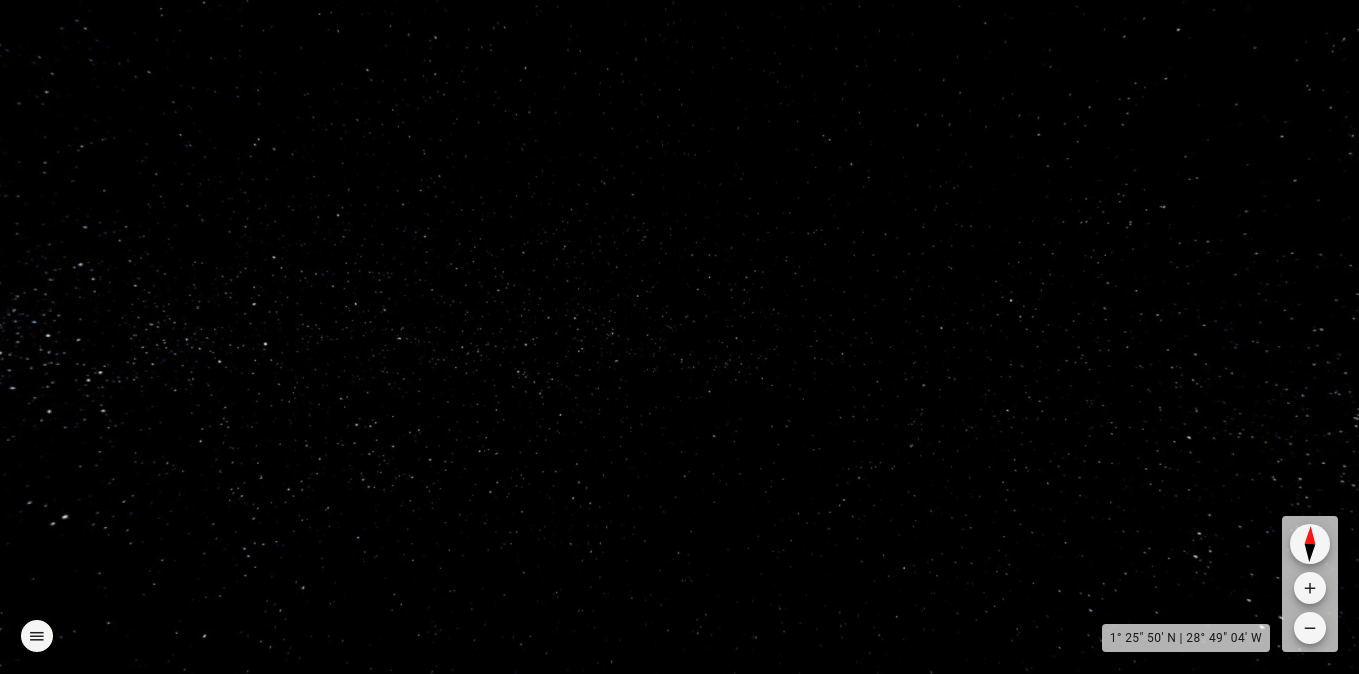
\includegraphics[width=\linewidth]{img/c4_starsVis.png}
  \caption{Wizualizacja gwiazd - klasa \texttt{StarsVis}}
  \label{fig:c4_starsVis} 
\end{figure}

Na listingu~\ref{lst:starsVis} pokazano część klasy \texttt{StarsVis} definiującą tę wizualizację. Kula tworzona jest z~użyciem klasy \texttt{THREE.SphereGeometry}, a~jej materiał \texttt{THREE.MeshBasicMaterial} zawiera ustawienia definiujące jej wyświetlanie. Ustawienie \mbox{\texttt{side:THREE.BackSide}} sprawia, że teksturowane są odwrotna niż zwykle strona rysowanego trójkąta. Ustawienia \mbox{\texttt{depthWrite:false}} oraz \mbox{\texttt{depthFunc:THREE.NeverDepth}} sprawiają, że obiekt nie będzie wpływał na wartość z-bufora, oraz będzie rysowany zawsze za innymi obiektami, co jest oczekiwane od obiektu tła. 


\begin{lstlisting}[float, language=javascript, label={lst:starsVis}, caption={
  Fragmenty klasy \texttt{StarsVis}}
]
/* ... */
export default class StarsVis extends Visualization {
private stars = new THREE.SphereGeometry(40000, 10, 10);
private starsMaterial = new THREE.MeshBasicMaterial({
  side: THREE.BackSide,
  map: new THREE.TextureLoader().load(starsMap),
  depthWrite: false,
  depthFunc: THREE.NeverDepth,
});
private mesh = new THREE.Mesh(this.stars, this.starsMaterial);
/* ... */
public setupCamera(camera: TrackballCamera): void {
  //
}
public setupScene(scene: THREE.Scene, group: THREE.Group): void {
  this.mesh.renderOrder = 0;
  group.add(this.mesh);
}
public update(deltaFactor: number): void {
  this.mesh.rotation.y = TimeService.getHourAngle();
}
/* ... */
}
\end{lstlisting}

Obiekt 3D \texttt{THREE.Mesh} w~metodzie \texttt{update} obracany jest w~osi $OY$ o~pewien kąt. Kąt ten wynika z~czasu słonecznego, ponieważ wizualizacja ta domyślnie ma stanowić tło dla wizualizacji Ziemi w~czasie rzeczywistym. Może być ona również rozszerzona, aby obsługiwać każdy inny dowolny czas. Kiedy kamera jest nieruchowa względem punktu na Ziemi, jej obrót w~okół własnej osi widoczny jest jako obrót tła w~przeciwnym kierunku. Klasa TimeService, dokładniej opisana w~dalszej części pracy, zawiera metodę \texttt{getHourAngle}, która dla danej strefy czasowej oblicza kąt obrotu słońca od danej długości geograficznej o~danym czasie~\cite{SolarTime}. Punktem odniesienia jest południk $\ang{0}$ i~strefa czasowa \textit{+00:00}. 

\section{Atmosfera}

Wizualizacja atmosfery stanowi wizualną dekorację dla innych wizualizacji. Składa się ona z~dwóch osobno generowanych części. Wizualnie atmosfera to poświata widoczna nad powierzchnią planety, która zanika wraz ze wzrostem wysokości punktu nad powierzchnią. Na efekt też wpływa sama grubość atmosfery, jej skład chemiczny, oraz gęstość w~poszczególnych jej partiach.

Utworzona wizualizacja nie posiada rozbudowanych możliwości konfiguracji i~została stworzona do współpracy z~wizualizacją Ziemi w~dużej skali. Na efekt poświaty składają się dwa obiekty. Pierwszym jest kula, której średnica odpowiada średnicy planety razem z~grubością atmosfery. Wyświetlana jest jej wewnętrzna część i~znając pozycje obserwatora, wyświetlana jest właściwie zanikająca poświata. Drugim obiektem jest kula rozmiarów planety, która zawsze generowana jest przed nią i~odpowiada za poświatę widoczną bezpośrednio nad planetą. Na rysunku~\ref{fig:c4_atmosphereVis} przedstawiono efekt atmosfery bez planety. Istotne są tutaj jedynie krawędzie widocznego okręgu, ponieważ jego środek ukryty będzie za planetą. Na rysunku~\ref{fig:atmosphere} przedstawiono schemat elementów kluczowych dla wyliczenia parametrów atmosfery. Kamera znajduje się w~punkcie $c_l$. Okrąg rysowany linią ciągłą symbolizuje powierzchnię planety, a~linią przerywaną, zasięg atmosfery. Wektor $\vv t$ stanowi przedłużenie wektora $\vv{g_v}$ o~grubość atmosfery. Widoczny dla obserwatora fragment atmosfery jest łukiem pomiędzy punktami $c_{gtb}$~i~$c_{gt}$.

\begin{figure}
\centering
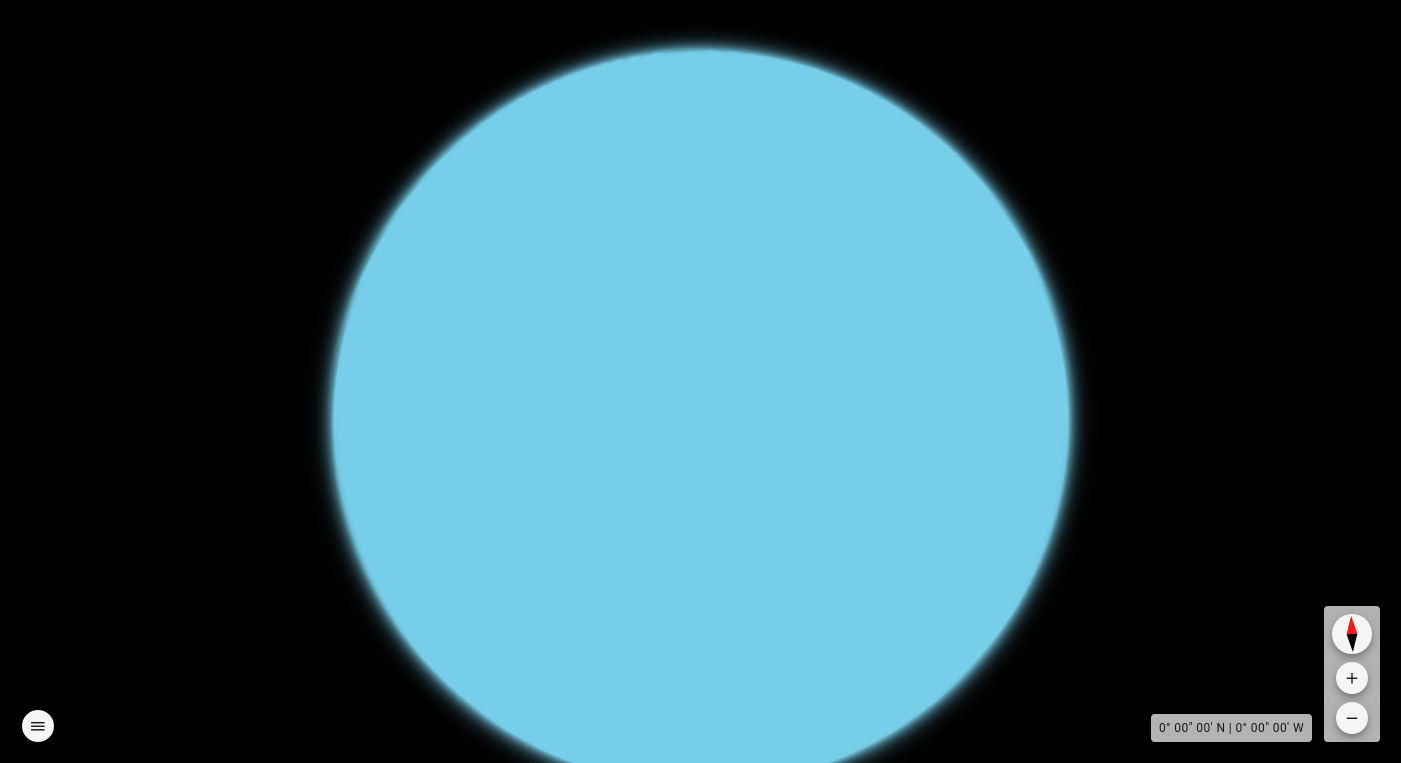
\includegraphics[width=\linewidth]{img/c4_atmosphereVis.png}
\caption{Wizualizacja atmosfery - klasa \texttt{AtmosphereVis}}
\label{fig:c4_atmosphereVis} 
\end{figure}

\begin{figure}[h]
\centering
\newlength{\gRadius}
\setlength{\gRadius}{3cm}
\newlength{\atmThickness}
\setlength{\atmThickness}{1cm}
\begin{tikzpicture}[scale=1.5]

    \coordinate (G) at (65:\gRadius);
    \coordinate (GT) at (65:\gRadius+\atmThickness);
    \coordinate (camera) at (90:\gRadius + \atmThickness + 1cm);
    \coordinate (center) at (90:0);
    \coordinate (atmTangent) at (126.869897646:\gRadius + \atmThickness);
    \coordinate (gTangent) at (143.130102354:\gRadius);
    \coordinate (atmBackTangent) at (184.539722109:\gRadius + \atmThickness);

    \draw[thick] circle (\gRadius);
    \draw[thick,dashed] circle (\gRadius+\atmThickness);
    \draw[red, fill=red] (0,5cm) circle (5pt);
    \draw[->] (center) -- (camera) node[midway,above,sloped] {\tiny$\vec G + \vec L$};
    \draw[->] (center) -- (G) node[midway,above,sloped] {\tiny$\vec G$};
    \draw[->] (G) -- (GT) node[midway,above,sloped] {\tiny$\vec T$};
    \draw[->] (G) -- (camera) node[midway,above,sloped] {\tiny$\vec L$};
    \draw[dashed] (camera) -- (atmTangent);
    \draw[dashed] (camera) -- (gTangent);

    \draw[->] (center) -- (atmTangent) node[midway,below,sloped] {\tiny$\vec G + \vec T$ };
    \draw pic["$\alpha$",draw=blue,thick,blue, ->, angle eccentricity=1.2, angle radius = 1.3cm]  {angle=camera--center--atmTangent};
    \draw pic["$\cdot$",draw, -, angle eccentricity=0.5, angle radius = 0.4cm]  {angle=center--atmTangent--camera};

    \draw[->] (center) -- (gTangent) node[midway,below,sloped] {\tiny$\vec G$ };
    \draw pic["$\beta$",draw=orange,thick,orange, ->, angle eccentricity=1.2, angle radius = 1.8cm]  {angle=camera--center--gTangent};
    \draw pic["$\cdot$",draw, -, angle eccentricity=0.5, angle radius = 0.4cm]  {angle=center--gTangent--camera};

    \draw[dashed] (gTangent) -- (atmBackTangent);
    \draw pic["$\cdot$",draw, -, angle eccentricity=0.5, angle radius = 0.4cm]  {angle=atmBackTangent--gTangent--center};
    \draw pic["$\gamma$",draw=red,thick,red, ->, angle eccentricity=1.2, angle radius = 1cm]  {angle=gTangent--center--atmBackTangent};
    \draw[->] (center) -- (atmBackTangent) node[midway,below,sloped] {\tiny$\vec G + \vec T$ };

\end{tikzpicture}


\caption{Schemat elementów kluczowych dla wyliczenia parametrów atmosfery}
\label{fig:atmosphere}
\end{figure}

\begin{lstlisting}[float, language=javascript, label={lst:atmosphereVis}, caption={
Fragmenty klasy \texttt{StarsVis}}
]
public atmosphereMaterial = new THREE.ShaderMaterial({
vertexShader: vertexShader,
fragmentShader: fragmentShader,
uniforms: {
  start: { value: 1 },
  stop: { value: 0.6 },
  fadeOut: { value: 0 },
  light: { value: 0 },
  power: { value: 1.25 },
  glowColor: { value: new THREE.Color(0x87ceeb) },
  viewVector: { value: new THREE.Vector3() },
  ...THREE.UniformsLib.lights,
},
depthFunc: THREE.NeverDepth,
lights: true,
transparent: true,
side: THREE.BackSide,
depthWrite: false,
});
\end{lstlisting}

Na listingu~\ref{lst:atmosphereVis} przedstawiono inicjalizację materiału odpowiedzialnego za poświatę nad planetą. Klasa \texttt{THREE.ShaderMaterial} pozwala kontrolować cały proces rysowania punktów, ponieważ wymaga dostarczenia obydwu typów shaderów. Tak jak w~przypadku materiału w~wizualizacji \texttt{StarsVis}, materiał definiuje też ustawienia modyfikacji z-bufora i~strony wyświetlanego trójkąta. Materiał definiuje również stałe dla jednego procesu rysowania (\texttt{uniforms}). Stałe te są aktualizowane w~każdym cyklu animacji. 
W procesie rysowania poświata generowana jest w~zależności od kąta pomiędzy wektorem normalnym płaszczyzny dla wierzchołka, a~wektorem określającym kierunek obserwacji. Niżej opisano stałe przekazywane do materiału.

\subsubsection{Uniform \texttt{start}}
Uniform \texttt{start} to ułamek liczby $\pi$ w~zakresie $\lbrack0; 1\rbrack$, który stanowi kąt wektora obserwatora z~wektorem normalnym wierzchołka, od którego rozpoczyna się rysowanie poświaty. Wartość ta zawsze wynosi $1$, co oznacza, że poświata rysowana jest od wierzchołków najdalej od kamery. Jego wektor normalny na rysunku \ref{fig:atmosphere} oznaczony został symbolem $\vv n$. Kąt między nim, a~wektorem $\vv{g_v} + \vv{l_v}$ wynosi $\ang{180}$, czyli $1 \cdot \pi$.

\subsubsection{Uniform \texttt{stop}}
Uniform \texttt{stop} to ułamek liczby $\pi$ w~zakresie $\lbrack0; 1\rbrack$, który stanowi kąt wektora obserwatora z~wektorem normalnym wierzchołka, od którego kończy się rysowanie poświaty o~pełnej przezroczystości. Ostatnim widocznym z~kamery punktem jest punkt $c_{gtb}$. Dalsza część schowana jest za planetą. Kąt ten wyliczany jest z~zależności $\beta+\gamma$. Sposób wyliczenia poszczególnych kątów pokazano na równaniach~\ref{eq:atm_beta}~i~\ref{eq:atm_gamma}.

\begin{align}
  \label{eq:atm_alfa}
  \alpha &= acos(\frac{\length{\vv{g_v}+\vv{t}}}{\length{\vv{g_v}+\vv{l_v}}}) \\
  \label{eq:atm_beta}
  \beta &= acos(\frac{\length{\vv{g_v}}}{\length{\vv{g_v}+\vv{l_v}}}) \\
  \label{eq:atm_gamma}
  \gamma &= acos(\frac{\length{\vv{g_v}}}{\length{\vv{g_v}+\vv{t}}})
\end{align}


\subsubsection{Uniform \texttt{fadeOut}}
Uniform \texttt{fadeOut} to ułamek liczby $\pi$ w~zakresie $\lbrack0; 1\rbrack$, który stanowi kąt wektora obserwatora z~wektorem normalnym wierzchołka, od którego kończy się rysowanie poświaty o~zanikającej przezroczystości. Jest ona interpolowana z~wykorzystaniem funkcji wygładzającej \texttt{expoIn}, którą pokazano na wykresie na rysunku~\ref{fig:c4_expoIn}. Kąt ten wyliczany jest z~zależności $\beta+\gamma-\alpha$.
\begin{figure}[h]
  \centering
  \begin{tikzpicture}[scale=0.7]
      \begin{axis}[domain=0:1,xmin=0,xmax=1.1,ymin=0,ymax=1.1,xlabel=$t$, ylabel=$f(t)$, legend pos=north west, width=0.6\textwidth, height=0.5\textwidth]
          \addplot[blue, ultra thick] {pow(2, 10 * x - 10)};
          \addlegendentry[text depth=2.5ex]{
              $f(t) = 
              \begin{cases}
                0 & \text{dla } t = 0\\
                2^{10 \cdot t - 10} & \text{dla } t > 0
              \end{cases}
              $
          };
      \end{axis}
  \end{tikzpicture}
  \caption{Funkcja wygładzająca \textit{expoIn}}
  \label{fig:c4_expoIn}
\end{figure}
\subsubsection{Uniform \texttt{light}}
Uniform \texttt{light} to ułamek liczby $\pi$ w~zakresie $\lbrack0; 1\rbrack$, który stanowi kąt przesunięcia oświetlanej powierzchni dla światła. Jeśli do sceny zostanie dodane światło kierunkowe to wpływa ono na wygląd atmosfery. W~normalnej sytuacji światło kierunkowe oświetla dokładnie pół kuli. Załóżmy sytuację, w~której kąt padania światła wyznacza wektor rozciągnięty pomiędzy punktami $c'_g$~i~$c_{gtb}$. W~takiej sytuacji atmosfera oświetlona by była na łuku pomiędzy wektorami $\vv {g'''_v}$~i~$\vv {g'_v} + \vv{t'_v}$. Żeby oświetlić pozostałą, widoczną część atmosfery (łuk pomiędzy punktami $c_{gtb}$~i~$c_{gt}$) w~obliczeniach, trzeba uwzględnić kąt $\gamma$.

\subsubsection{Uniform \texttt{power}}
Uniform \texttt{power} to wykładnik potęgi, do której podniesiona zostaje finalna przezroczystość materiału atmosfery, przed kalkulacją oświetlania. Wartość ta nie jest aktualizowana i~wynosi $1.25$.

\subsubsection{Uniform \texttt{glowColor}}
Uniform \texttt{glowColor} to bazowy kolor materiału atmosfery. Nie ulega on zmianie i~ma wartość \texttt{0x87ceeb}. Możliwą poprawą zachowania atmosfery byłaby dynamiczna zmiana koloru atmosfery powiązana z~kątem padania światła, co symulowałoby zmianę koloru w~miejscach zachodu i~wschodu słońca.

\subsubsection{Uniform \texttt{viewVector}}
Uniform \texttt{viewVector} to wektor jednostkowy skierowany od środka $s$ grupy obrotu do kamery $c_l$. Odpowiada on za orientację wyświetlanej atmosfery zawsze w~kierunku punktu, w~którym znajduje się kamera. Uzyskanie wektora przed normalizacją przedstawiono na równaniu~\ref{eq:c4_atm_1}.

\begin{equation}
  \label{eq:c4_atm_1}
  \vv v = q^{-1}([0, 0, \length{\vv{g_v}}]^T + \vv{l_v})q
\end{equation}
\begin{eqexpl}[25mm]
\item {$\vv v$} wektor \texttt{viewVector}
\item {$q$} kwaternion uzyskany z~macierzy układu odniesienia wizualizacji. W~równaniu obrót następuje w~kierunku odwrotnym.
\end{eqexpl}

Uniform \texttt{fadeOut} bierze też udział w~ujednoliceniu koloru nieba, kiedy kamera schodzi poniżej granicy atmosfery. Zachowanie to nie zostało jednak wystarczająco rozwinięte, żeby odzwierciedlać realistycznie przejście pomiędzy czernią kosmosu, a~niebieskim niebem z~użyciem tego samego matariału w~procesie rysowania. Pozostałe stałe w~opisywanym materiale są uzupełnieniem z~obiektu \mbox{\texttt{THREE.UniformsLib.lights}}. Zawierają one dane związane ze światłami obecnymi na scenie. 

Materiał opisujący wygląd drugiej kuli, atmosfery widocznej nad ziemią, ma podobną budowę, korzysta z~wyliczonych kątów i~podobnych mechanizmów. Biorąc to pod uwagę, nie zostanie on tutaj opisany. 

\section{Ziemia}

Opisane wcześniej wizualizacje kosmosu i~atmosfery pozwalają na stworzenie wizualizacji planety. Wizualizacja \texttt{EarthVis} jest wizualizacją planety Ziemi, która prezentuje jej aktualne oświetlenie przez Słońce. Widok początkowy wizualizacji przedstawiono na rysunku~\ref{fig:c4_earthVis_1}. 


\begin{figure}[h]
  \centering
  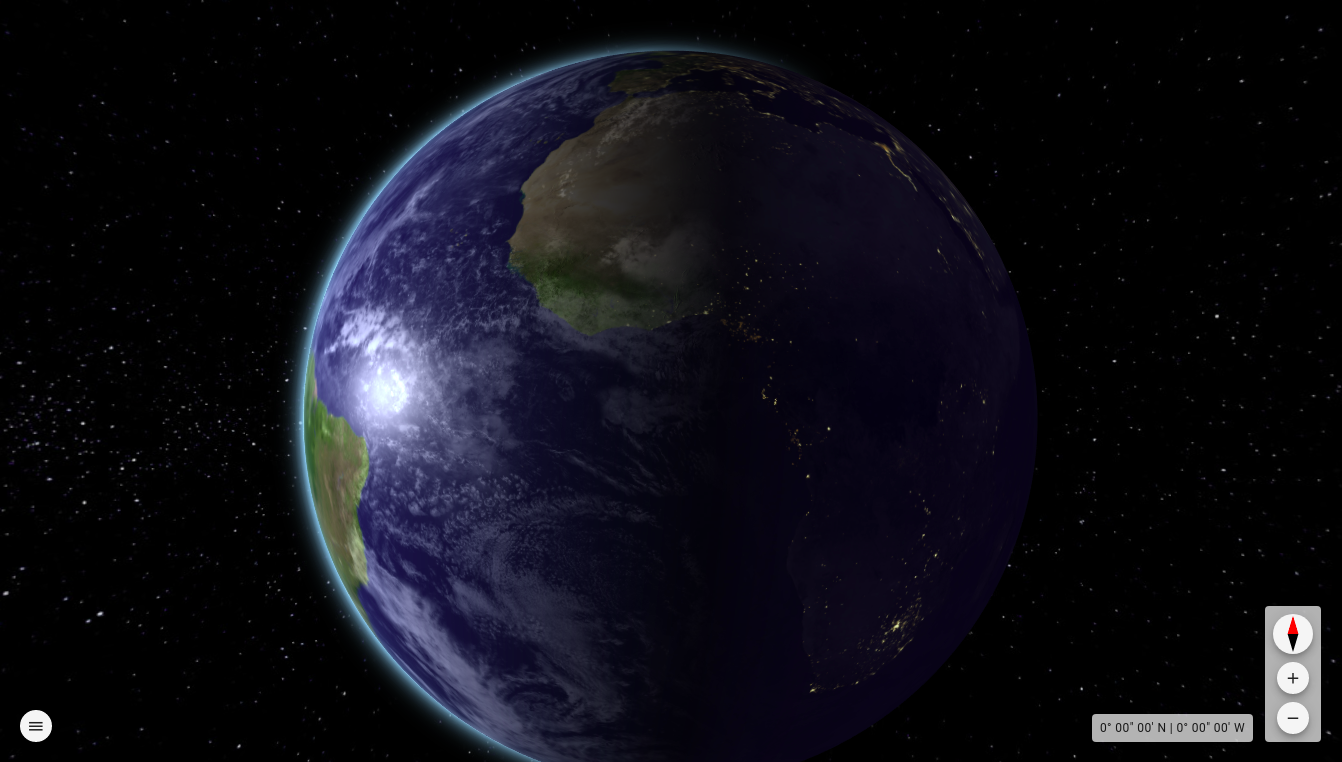
\includegraphics[width=\linewidth]{img/c4_earthVis_1.png}
  \caption{Widok początkowy wizualizacji Ziemi o~godzinie 19:50, 27.09.2020r.}
  \label{fig:c4_earthVis_1} 
\end{figure}
  

\begin{figure}[h]
  \centering
  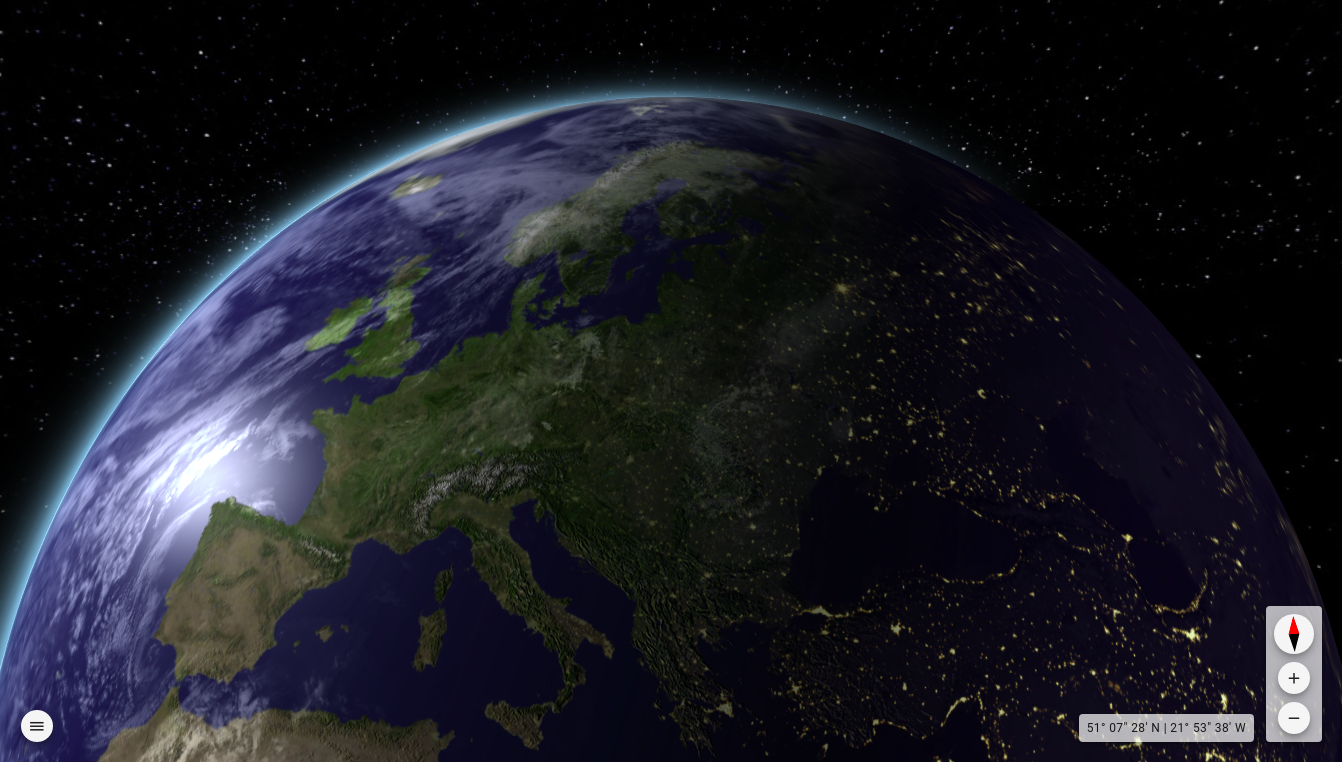
\includegraphics[width=\linewidth]{img/c4_earthVis_2.png}
  \caption{Zachód słońca nad Europą o~godzinie 18:54, 27.07.2020r.}
  \label{fig:c4_earthVis_2} 
\end{figure}
  
Podczas każdej aktualizacji animacji obliczane jest nowe położenie słońca. Poruszając się w~układzie odniesienia Ziemi konieczne jest obliczenie deklinacji Słońca, czyli kąta pomiędzy nim, a~płaszczyzną równika~\cite{Declination}. Drugą wartością konieczną do wyliczenia jest kąt godzinny~\cite{SolarTime}. Jest to kąt, o~jaki obróciło się Słońce od wybranego punktu odniesienia dla wybranej strefy czasowej w~konkretnej chwili. Wizualizacja Ziemi stanowi podstawę do wizualizacji połączonych z~nią zjawisk dużej skali. Bazują na niej wizualizacje \texttt{ActiveSatellitesVis} oraz \texttt{IssVis} opisane w~dalszej części pracy. Na rysunku~\ref{fig:c4_earthVis} przedstawiono diagram zależności pomiędzy poszczególnymi wizualizacjami i~klasami pomocniczymi.

\begin{figure}
  \centering
  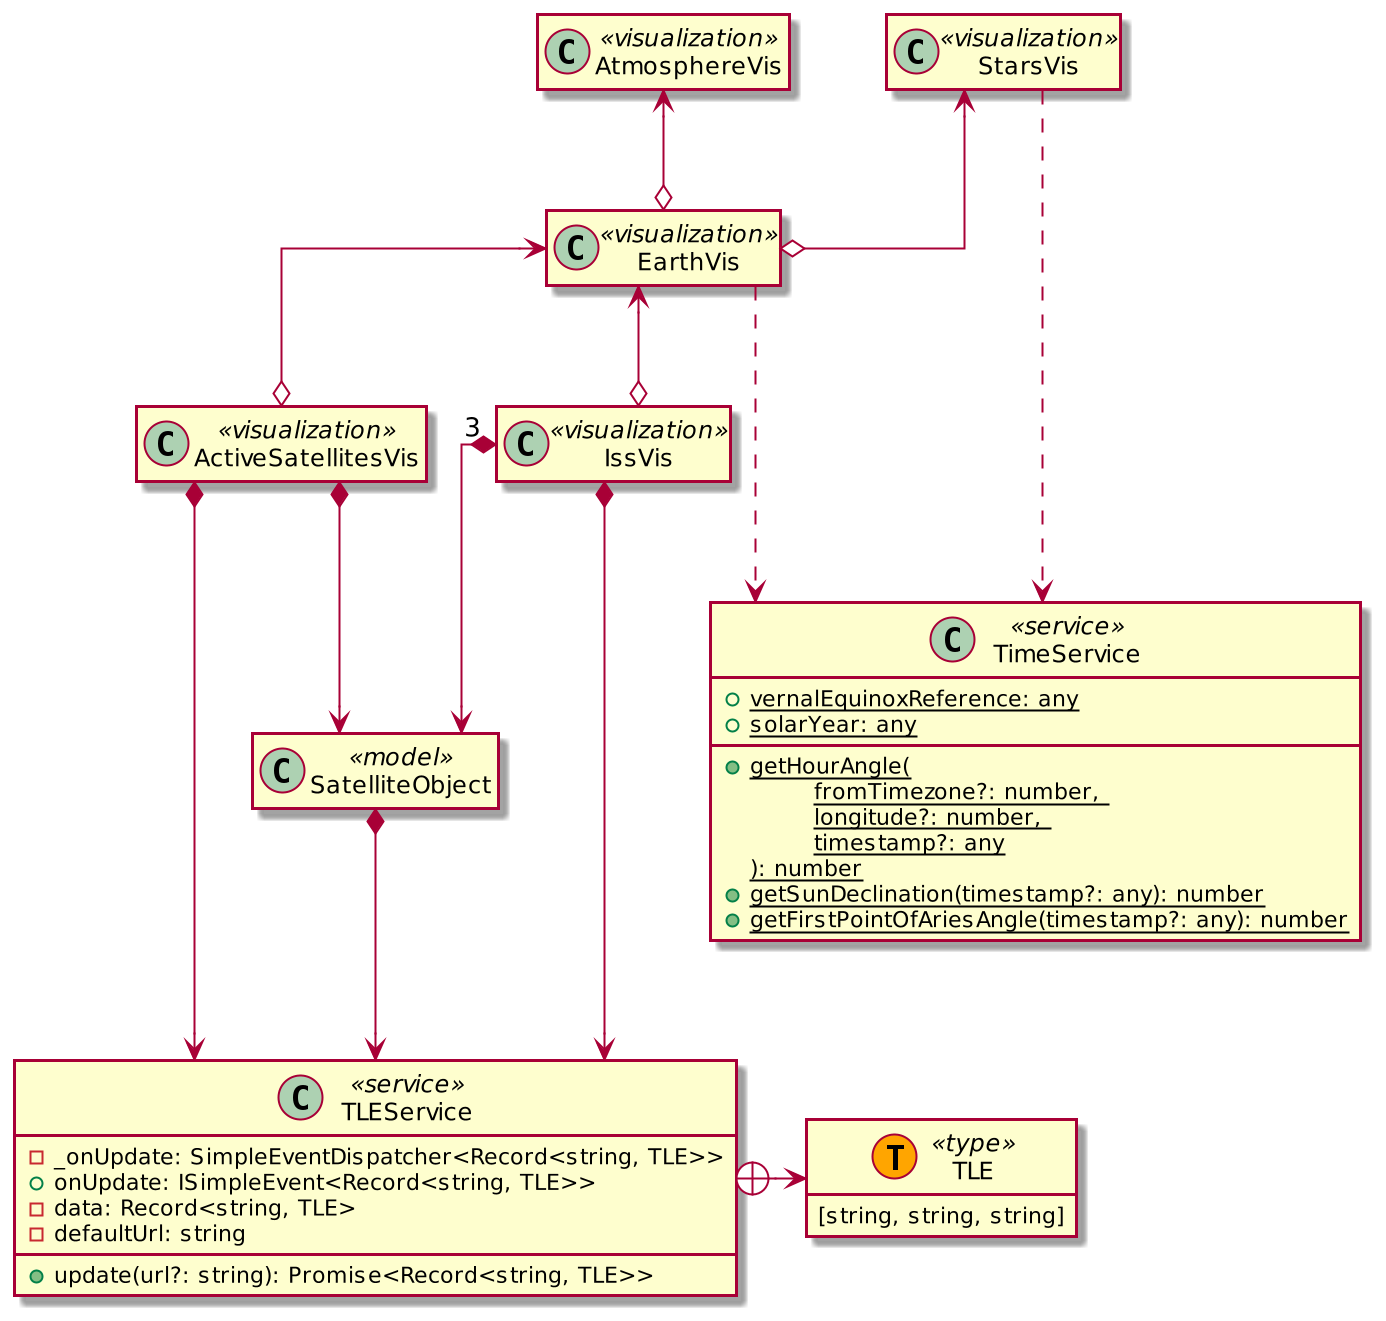
\includegraphics[width=\textwidth]{diagrams/out/c4_earthVis.png}
  \caption{Zależności pomiędzy klasami wizualizacji Ziemi}
  \label{fig:c4_earthVis} 
\end{figure}

Na wizualizację składają się wszystkie obiekty ustawiane przez wizualizacje \texttt{AtmosphereVis} i~\texttt{StarsVis}. Na scenie w~układzie współrzędnych wizualizacji znajdują się dwie kule. Pierwsza z~nich odpowiada za wyświetlanie tekstury Ziemi, a~druga, z~promieniem większym o~$4$~km, wyświetla chmury. Materiał pierwszej kuli implementuję model oświetlanie mz cieniowaniem Phonga~\cite[Rozdział 3]{RealTime3DGraphics} za pomocą obiektu \texttt{THREE.MeshPhongMaterial} i~używa trzech map.
\begin{samepage}
\begin{enumerate}
  \item \texttt{map} - mapa zawierająca kolor tekseli tekstury
  \item \texttt{specular map} - mapa zawierająca poziom odbicia kierunkowego światła dla każdego teksela tekstury
  \item \texttt{normalMap} - mapa zawierająca wektory normalne w~przestrzeni stycznej wierzchołka modelu.
\end{enumerate}
\end{samepage}
Materiał kuli wyświetlające chmury zawiera tylko mapę definiującą sam kolor tekseli. Jako, że ta mapa jest obrazem chmur na czarnym tle i~nie zawiera kanału \texttt{alpha}, materiał w~procesie renderowania stosuje mieszanie addytywne. Grupa obrotu zawiera również światło kierunkowe, które zawsze skierowane jest do jej środka. Pozycja źródła światła obracana jest zgodnie z~wartościami wyliczonymi przez serwis \texttt{TimeService}, kolejno o~kąt godzinny w~osi~$OY$ i~deklinację w~osi~$OX$.

Na rysunku~\ref{fig:c4_earthVis_2} pokazane zostało płynne przejście pomiędzy teksturą nocną i~dzienną, która jest wyświetlana w~zależności od oświetlenia planety. Zachowanie to wymagało zmodyfikowania domyślnego fragment shadera i~uzależnienia wyświetlanej tekstury od kąta pomiędzy interpolowanym wektorem normalnym dla teksela, a~kierunkiem padania światła. Na listingu~\ref{lst:earthFrag} pokazano najważniejszą część modyfikacji shadera. Potrzebny kąt wyliczany jest z~wykorzystaniem iloczynu skalarnego wspomnianych wektorów. Wynik ten musi być zmapowany z~przedziału $\lbrack-1; 1\rbrack$ na przedział $\lbrack0; 1\rbrack$. Obliczenie wartości, która trafia do funkcji wygładzającej, a~następnie do funkcji \texttt{mix}, która miesza wartości tekseli, pokazano na równaniu~\ref{eq:earth_dot}.

\begin{lstlisting}[float=h, language=C++, label={lst:earthFrag}, caption={
  Modyfikacja fragment shadera materiału \texttt{MeshPhongMaterial}}
]
#if NUM_DIR_LIGHTS > 0
  float dotL =  dot(vNormal, directionalLights[0].direction);
  vec4 texelColorNight = texture2D( nightMap, vUv );
  texelColorNight = mapTexelToLinear( texelColorNight );

  outgoingLight = mix(
    vec3(texelColorNight) + ambientLightColor,
    outgoingLight,
    easeInOutExpo(dotL*0.5+0.5)
  );
#endif
\end{lstlisting}
\begin{equation}
  \label{eq:earth_dot}
  x = (\vv{n} \cdot \vv{d}) \cdot 0.5 + 0.5
\end{equation}
\begin{eqexpl}[25mm]
\item {$\vv n$} wektor normalny
\item {$\vv d$} kierunek padania światła
\item {$x$} wartość w~przedziale $\lbrack0; 1\rbrack$
\end{eqexpl}
\vspace{\baselineskip}

Wizualizacje dostarcza również panel kontrolny, który pokazany został na rysunku~\ref{fig:c3_controls_earth} i~pozwala na przełączanie się pomiędzy trybami kamery - swobodnym i~kompas.

\section{Wybrane satelity}

Wizualizacją stworzoną na podstawie wizualizacji Ziemi jest wizualizacja wybranych satelitów orbitujących wokół niej. Klasą definiującą tę wizualizację jest klasa \texttt{IssVis} obecna na rysunku~\ref{fig:c4_earthVis}. Znajdują się na nim również klasy wspomagające wyświetlanie i~wyliczanie pozycji obiektów. Na scenie znajdują się trzy satelity. Są nimi Międzynarodowa Stacja Kosmiczna, Kosmiczny Teleskop Hubble'a oraz Eutelsat Hot Bird 13C. Każda satelita reprezentowana jest za pomocą trzech obiektów, którymi jest elipsa reprezentująca kształt orbity, obiekt satelity będący złożonym modelem 3D lub sferą oraz linia łącząca obiekt satelity ze środkiem planety.  Wizualizacja dostarcza komponent panelu kontrolnego, który umożliwia zmianę trybu pracy kamery oraz zarządzenie widocznością poszczególnych satelitów. Pozycja satelitów wyświetlana jest w~czasie rzeczywistym, a~ich pozycja i~orbita kalkulowana jest z~wykorzystaniem danych w~formacie TLE~(ang.~Two-Line Elements).

\subsection{TLE}
TLE jest formatem zapisu informacji o~satelicie pozwalającym wyznaczyć z~dużym przybliżeniem jej pozycję relatywnie do ciała orbitowanego~\cite{TLE}. Pierwsza linia zawiera nazwę satelity i~może być pomijana w~zapisie. Druga linia jednoznacznie identyfikuje satelitę i~zawiera informacje o~punkcie w~czasie, dla którego określone są parametry orbity - epokę. Zawiera również informacje kontrolne o~samym TLE oraz pierwszą i~drugą pochodną prędkości ruchu. Trzecia linia zawiera parametry orbity. Najważniejszymi z~nich są inklinacja, kąt węzła wstępującego, ekscentryczność i~argument perycentrum, który dla Ziemi nazywa się argumentem perygeum. Poniżej przedstawiono przykładowe dane dla Międzynarodowej Stacji Kosmicznej.
\begin{verbatim}
ISS (ZARYA)
1 25544U 98067A   08264.51782528 -.00002182  00000-0 -11606-4 0  2927
2 25544  51.6416 247.4627 0006703 130.5360 325.0288 15.72125391563537
\end{verbatim}

W stworzonej wizualizacji TLE pobierane są ze strony CelesTrak~\cite{CelesTrak}, która zbiera i~analizuje dane otrzymane od jednostki NORAD (ang. North American Aerospace Defense Command). Dane otrzymywane są w~formacie tekstowym. Serwis \texttt{TLEService} odpowiedzialny jest za pobranie danych TLE wszystkich aktywnych satelit, sparsowanie je, a~następnie wyemitowanie zdarzenia \texttt{onUpdate}, które może być obsłużone w~procesie inicjalizacji obiektów na scenie. Serwis ten umożliwia również dostęp do danych satelity z~wykorzystaniem jej identyfikatora. Dla satelit, na których pozycję wpływać może atmosfera i~inne nieprzewidziane czynniki, dane TLE mogą z~czasem stawać się nieaktualne. Dzieje się to jednak na przestrzeni dni. Założyć można, że pobranie najnowszej ich wersji w~momencie uruchamiania wizualizacji pozwala na wystarczająco dokładne wyliczenia ich pozycji.

Za obliczenie parametrów orbity, wygenerowanie obiektów sceny i~odpowiednią transformację ich pozycji odpowiada obiekt \texttt{SatelliteObject} reprezentujący pojedynczą satelitę. Oblicza on parametry elipsy i~generuje reprezentujący ją obiekt klasy \texttt{THREE.EllipseCurve}. Równania~\ref{eq:sat_1}~-~\ref{eq:sat_3} opisują proces wyliczenia parametrów orbity. Wyliczenia półosi wielkiej $a$ wynika z~trzeciego prawa Kelpera, które łączy jej długość zależnością z~okresem obiegu satelity wokół Ziemi, który to dostarcza TLE. Transformacja aktualizowana jest w~każdym przebiegu pętli animacji.

\begin{samepage}
  \begin{figure}[h]
  \begin{align}
      \label{eq:sat_1}
      a~&= \frac{G^{\frac{1}{3}}}{(\frac{2n\pi}{86400})^{\frac{2}{3}}} \\
      \label{eq:sat_2}
      b &= a\sqrt{1-e^2} \\
      \label{eq:sat_3}
      c &= e \cdot a
  \end{align}
  \begin{eqexpl}[25mm]
      \item {$a$} półoś wielka orbity
      \item {$G$} standardowy parametry grawitacyjny Ziemi
      \item {$n$} średnia liczba obiegów Ziemi w~ciągu 24 godzin
      \item {$b$} półoś mała orbity
      \item {$e$} ekscentryczność orbity
      \item {$c$} przesunięcie od środka do ogniska orbity
  \end{eqexpl}
  \vspace{\baselineskip}
\end{figure}
\end{samepage}

Finalna transformacja obiektu elipsy jest z~złożeniem obrotów i~translacji. Najpierw wykonywana jest translacja elipsy tak, aby środek Ziemi pokrywał się z~jej ogniskiem. Następnie w~osi $OX$ elipsa obracana jest o~kąt wynikający z~danych o~inklinacji orbity.  Potem wykonywany jest obrót w~osi $OY$ o~kąt wynikający z~położenia punktu Barana, czyli punktu służącego do orientacji w~odniesieniu do równikowego układu współrzędnych oraz ekliptyki. W~tej samej osi elipsa obracana jest o~kąt wynikający z~kąta węzła wstępującego oraz o~kąt przeciwny do kąta godzinnego, aby uwzględnić obrót Ziemi w~czasie. Na końcu następuje obrót uwzględniający argument perygeum. 

Funkcja \texttt{TimeService.getFirstPointOfAriesAngle} odpowiedzialna jest za obliczanie kąta od punktu Barana. W~obecnej implementacji może ona jednak być czynnikiem wpływającym na brak pokrycia orientacji orbity w~osi $OY$ z~jej faktyczną trajektorią. Sztuczna korekcja staje się również nieaktualna po jakimś czasie. Autor wizualizacji nie był w~stanie dostatecznie zbadać przyczyny tego problemu. 

Za obliczanie pozycji samej satelity na orbicie odpowiada biblioteka \texttt{tle.js}~\cite{tle.js}, która jest używana w~procesie aktualizacji obiektu \texttt{SatelliteObject}. Pozwana ona, na postawie TLE, uzyskać położenie satelity o~podanym czasie. Etykiety generowane są z~użyciem obiektu \texttt{THREE.Sprite}, który wyświetla kwadratową teksturę zawsze zorientowaną w~kierunku obserwatora. Tekstura jest napisem, który rysowany jest dynamicznie na elemencie \texttt{Canvas} przetworzonym przez obiekt \texttt{THREE.CanvasTexture}. Rozmiar etykiet jest wprost proporcjonalny do odległości obiektu od obserwatora. Zachowanie to utrzymuje taki sam rozmiar etykiet niezależnie od orientacji kamery na scenie.

\begin{figure}
  \centering
  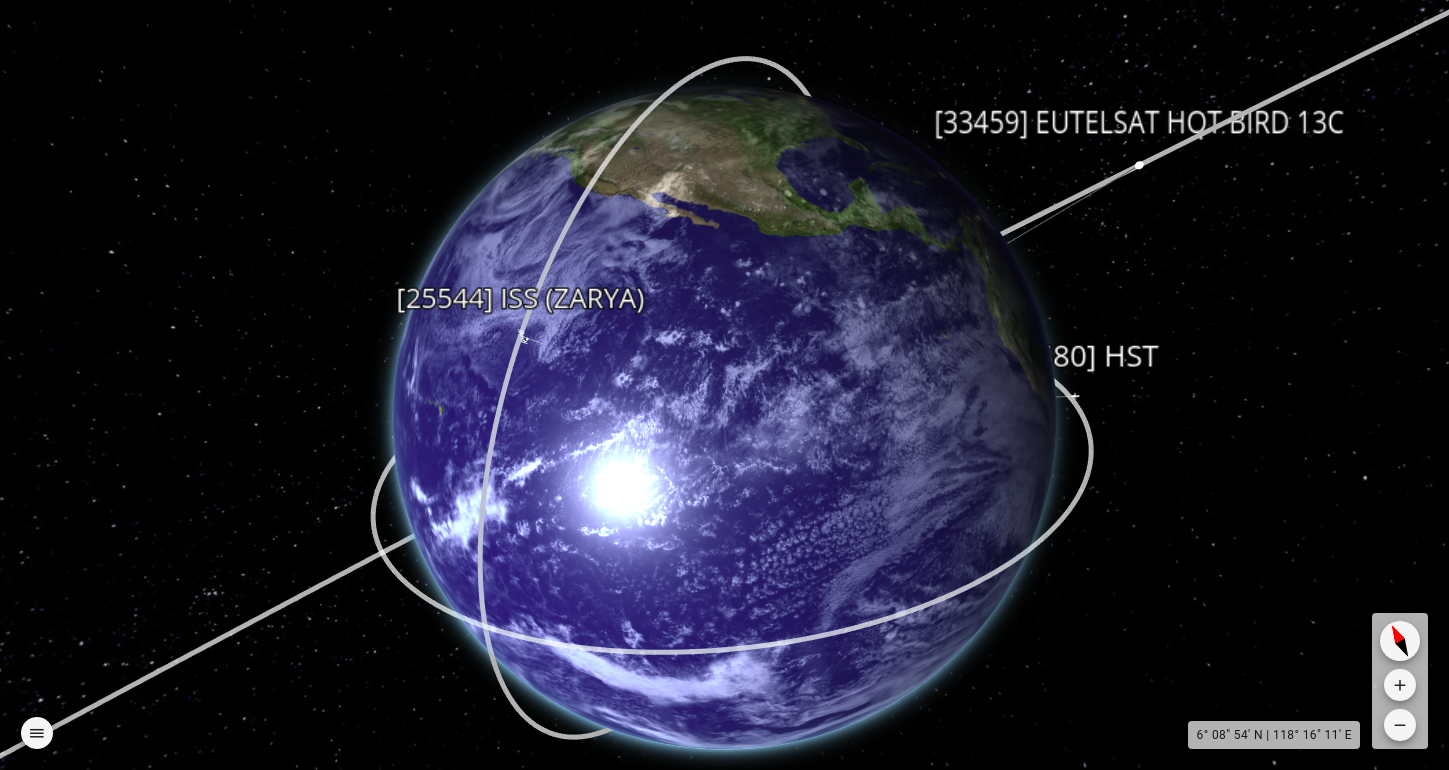
\includegraphics[width=\linewidth]{img/c4_issVis.png}
  \caption{Wybrane satelity - klasa \texttt{IssVis}}
  \label{fig:c4_issVis} 
\end{figure}

\section{Aktywne satelity}

Wizualizacja, którą opisuje klasa \texttt{ActiveSatellitesVis}, która pokazana jest na rysunku~\ref{fig:c4_earthVis}, wyświetla wszystkie aktywne satelity na podstawie danych ze strony CelesTrak~\cite{CelesTrak}. Widok początkowy wizualizacji przedstawia za pomocą punktów pozycje satelit w~chwili obecnej. Wizualizacja dostarcza panel kontrolny, dzięki któremu można zmienić tryb ruchu kamery oraz przyspieszyć upływ czasu. Można dzięki temu zobaczyć przybliżoną pozycję satelitów w~przyszłości. Panel kontrolny posiada również możliwość resetu czasu wizualizacji do chwili obecnej. Na rysunku~\ref{fig:c4_activeSatellitesVis} pokazana została wizualizacja oraz jej panel kontrolny. Widać na nim dobrze łuk, którą tworzą satelity na orbicie geostacjonarnej.

\begin{figure}
  \centering
  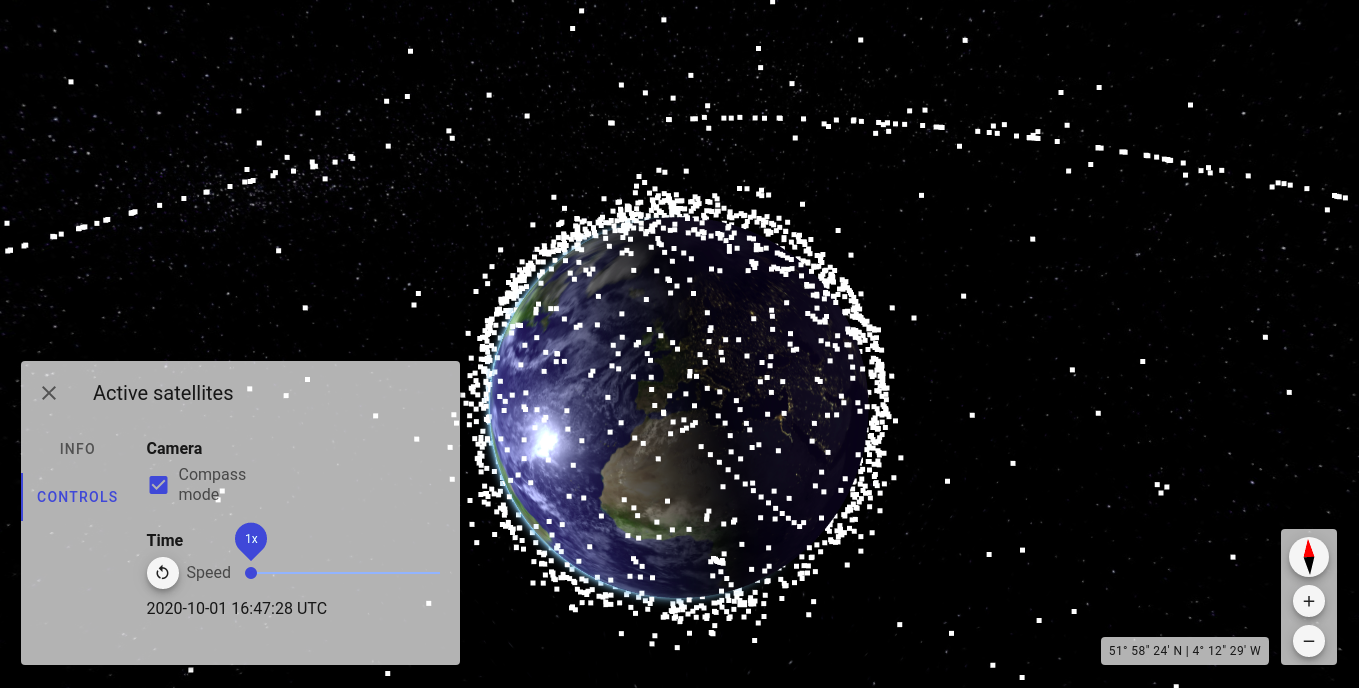
\includegraphics[width=\linewidth]{img/c4_activeSatellitesVis.png}
  \caption{Aktywne satelity - klasa \texttt{ActiveSatellitesVis}}
  \label{fig:c4_activeSatellitesVis} 
\end{figure}

Podobnie jak w~przypadku wizualizacji opisanej klasą \texttt{IssVis} dane TLE pobierane są i~zarządzane poprzez klasę \texttt{TLEService}. Kalkulacja pozycji satelitów również wykonywana jest z~użyciem mechanizmów klasy \texttt{SatelliteObject}. Różnicą pomiędzy tymi wizualizacjami jest to, że klasa \texttt{SatelliteObject} nie tworzy i~nie dodaje do sceny obiektów reprezentujących satelity. 

\begin{lstlisting}[float, language=javascript, label={lst:active1}, caption={
  Fragmenty klasy \texttt{ActiveSatellitesVis}}
]
private pointsMaterial = new THREE.PointsMaterial({
  transparent: true,
  color: 0xffffff,
  size: 5,
  sizeAttenuation: false,
});
private points = new THREE.Points(
  new THREE.BufferGeometry(),
  this.pointsMaterial
);

public update(deltaFrac: number) {
  /* ... */
  const points: number[] = [];
  this.sateliteObjects.forEach((o) => {
    const p = o.getPosition(this.timestamp);
    points.push(p.x, p.y, p.z);
  });
  this.points.geometry.setAttribute(
    "position",
    new THREE.BufferAttribute(new Float32Array(points), 3)
  );
  /* ... */
}
\end{lstlisting}

Dostępne dane zawierają informacje o~około 8000 aktywnych satelitów. Wywołanie polecenia rysowania dla każdego punktu oddzielnie skutkowałoby długim czasem rysowania, ponieważ w~procesie generowania grafiki najwięcej czasu tracone jest na komunikacji z~GPU. Dlatego wizualizacja wywołuje tylko jedno polecenie rysowania dla wszystkich punktów. Listing~\ref{lst:active1} zawiera inicjalizację obiektu materiału \texttt{THREE.PointsMaterial} oraz obiektu \texttt{THREE.Points} odpowiedzialnego za reprezentację punktów na scenie. Inicjalizowany jest on z~pustym buforem reprezentującym pozycje wierzchołków. Rola buforów w~procesie rysowania opisana została w~rozdziale~\ref{sec:render}. W~pokazanej na listingu~~\ref{lst:active1} metodzie \texttt{update}, wykonywanej co każde przejście pętli głównej, bufor uzupełniany jest nowymi współrzędnymi punktów. Wszystkie punkty rysowane są za pomocą jednego polecenia, a~rysowanie każdego z~osobna dzieje się równolegle w~GPU. Największy narzut obliczeniowy spowodowany jest kalkulacją pozycji w obiektach \texttt{SatelliteObject}, który przy dużych liczbach jest już dostrzegalny.

\section{Kafelki i Radar pogodowy}

% Co pokazuje, co może panel kontrolny
% wiele warstw konfigurowalnych

\begin{figure}
  \centering
  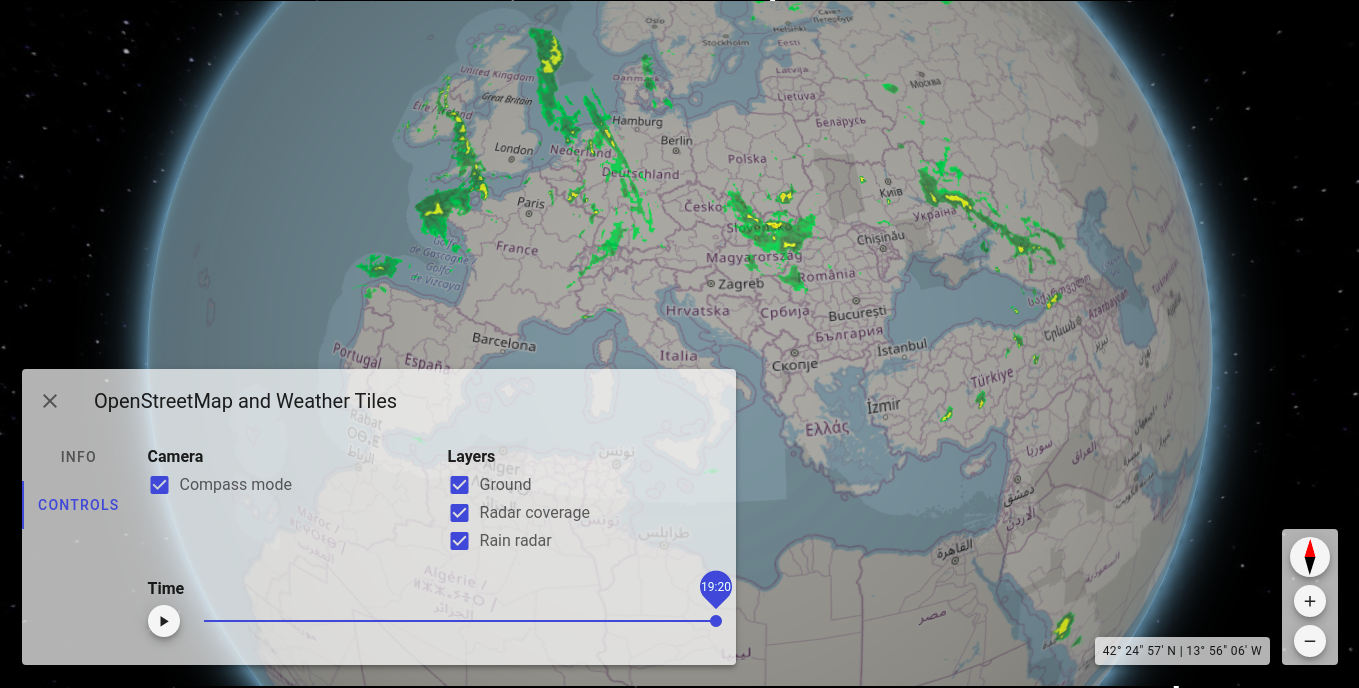
\includegraphics[width=\linewidth]{img/c4_osmTilesVis.png}
  \caption{Opady deszczu nad Europą - klasa \texttt{OsmTilesVis}}
  \label{fig:c4_osmTilesVis} 
\end{figure}

\begin{figure}
  \centering
  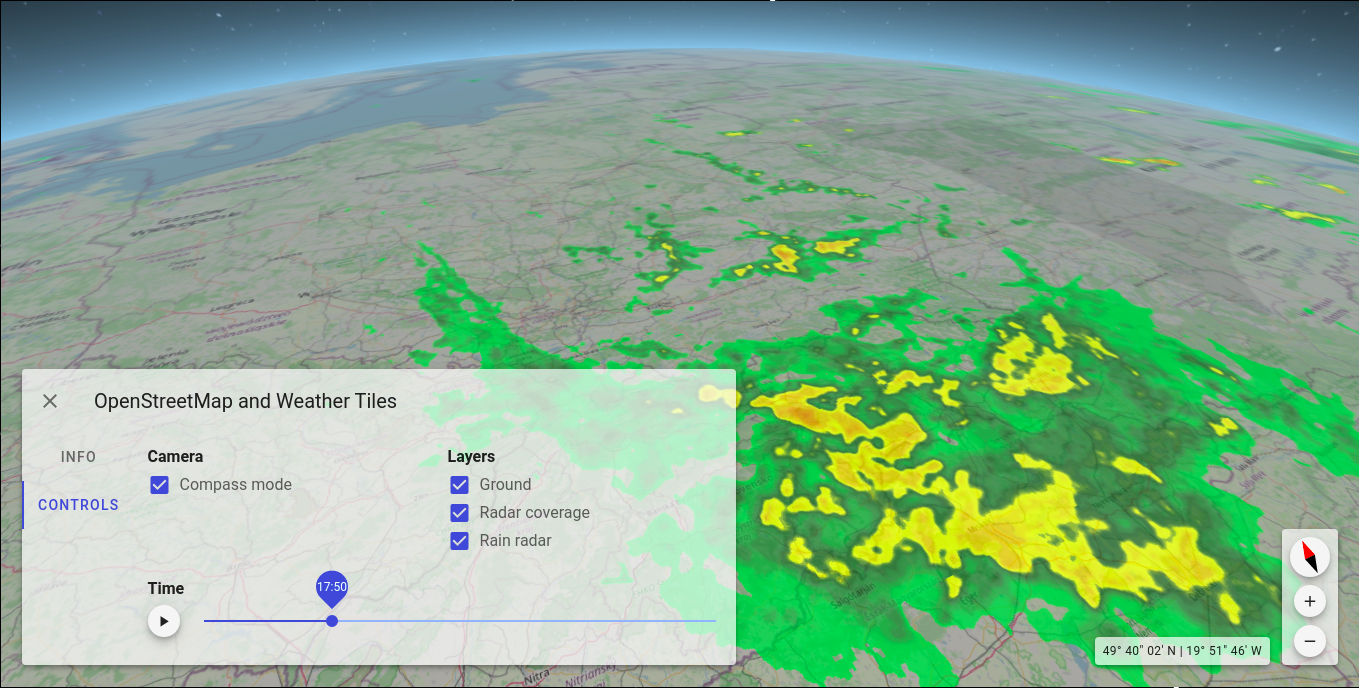
\includegraphics[width=\linewidth]{img/c4_osmTilesVis_1.png}
  \caption{Opady deszczu nad Polską - klasa \texttt{OsmTilesVis}}
  \label{fig:c4_osmTilesVis_1} 
\end{figure}

% Kafelki subsection
% Odwzorowanie map

% Implementacja subsection
% Diagram klas
